%%%%%%%%%%%%%%%%%%%%%%%%%%%%%%%%%%%%%%%%%%%%%%%%%%%%%%%%%%%
% | - Active Learning Machine Learning Results %%%%%%%%%%%%
% %%%%%%%%%%%%%%%%%%%%%%%%%%%%%%%%%%%%%%%%%%%%%%%%%%%%%%%%%
%
% Notes:
%   - QUESTION Is there any physical intuition that we can gleam from the fingerprints?
%     * Probably not important
%   - QUESTION What did @Chris mean by this? "Computed amorphous phase to define synthesizability"
%     * ANSWER: Referring to Murat's paper R85
%     * I don't think we can take advantage of this since there is no amorphous data for IrO3
% Mention that we have ~15 metastable structures inbetween rutile and anatase IrO2
% __| %%%%%%%%%%%%%%%%%%%%%%%%%%%%%%%%%%%%%%%%%%%%%%%%%%%%%



% %%%%%%%%%%%%%%%%%%%%%%%%%%%%%%%%%%%%%%%%%%%%%%%%%%%%%%%%%
% ####################### Paragraph #######################
% %%%%%%%%%%%%%%%%%%%%%%%%%%%%%%%%%%%%%%%%%%%%%%%%%%%%%%%%%
% Intro/transition paragraph
% | - %%%%%%%%%%%%%%%%%%%%%%%%%%%%%%%%%%%%%%%%%%%%%%%%%%%%%
%
We next utilized the active learning scheme to discover of the most stable forms of \IrOtwo and \IrOthree.
%
The algorithm is applied to each stoichiometry individually, and because both cases demonstrate the efficacy of the algorithm equally well, we will focus on walking through the algorithm for the more novel \IrOthree stoicheometry.
%
Will will briefly touch on the results for \IrOtwo at the end and refer the reader to the Supporting Information for further information.
% __| %%%%%%%%%%%%%%%%%%%%%%%%%%%%%%%%%%%%%%%%%%%%%%%%%%%%%

% %%%%%%%%%%%%%%%%%%%%%%%%%%%%%%%%%%%%%%%%%%%%%%%%%%%%%%%%%
% ####################### Paragraph #######################
% %%%%%%%%%%%%%%%%%%%%%%%%%%%%%%%%%%%%%%%%%%%%%%%%%%%%%%%%%
% Results for IrO3
% AL results for IrO3
%   * Introduce the convergence plots
%   * The GP becomes more accurate as more DFT is acquired
%   * The GP can start to recognize the low energy systems after minimal DFT
%   *
% We need to call them something else than "convergence plots" (bad name)
% | - %%%%%%%%%%%%%%%%%%%%%%%%%%%%%%%%%%%%%%%%%%%%%%%%%%%%%
%
Figure~\ref{fig:iro2_al}a shows a sequence of plots at various generations of the active learning algorithm applied to \IrOthree,
starting with the initial generation of five randomly drawn candidate structures and ending with the 40th generation
(\num{205} DFT computed structures out of the \num{248} total candidates).
%
% COMBAK Why are we sorting? Explain
Each plot reports the predicted (light grey) and DFT-derived (solid red) formation enthalpies ($y$-axis) for each structure sorted from most to least stable ($x$-axis).
%
As the algorithm acquires DFT data, the GP model becomes more accurate, as evidenced by the decreasing uncertainties when comparing the the initial generations to the latter generations of the AL (\ref{fig:iro2_al}a.i-v).
%
% \textbf{This is difficult to see in the figure, can you move the text inset down and make these lines longer?}
At the top of each subplot of Figure~\ref{fig:iro2_al} the identity of ten most stable polymorphs is tracked,
with the short grey line turning into a longer red line when the structure is acquired by the algorithm.
%
At the first generation the ten most stable structures are randomly distributed across the entire candidate space because the GP model has not been trained sufficiently to correctly identify the most stable polymorphs.
%
After only three generations (Figure~\ref{fig:iro2_al}a.ii) the GP model is sufficiently trained to predict all of the 10 most stable polymorphs as being low energy configurations, as evidenced by the fact that their predicted energy ordering within the candidate space has shifted towards the low energy portion of Figure~\ref{fig:iro2_al}a.ii.
%
By the third generation (\num{20} DFT calculations) \num{2/10} most stable polymorphs have been acquired.
%
% COMBAK Does this syntax work with num?
By the 6th generation (Figure~\ref{fig:iro2_al}a.iii) (\num{15} additional DFT calculations) the AL routine has successfully identified \num{7/10} of the lowest energy structures.
%
Figure~\ref{fig:iro2_al}e plots the quantity of the most stable ten systems acquired as a function of DFT calculations for the AL algorithm with the GP-UCB acquisition function and a baseline random acquisition scheme.
%
The results of Figure~\ref{fig:iro2_al}e are averaged over independent runs of AL algorithms with the 1 sigma standard deviation between these runs shown.
%
Overall, the GP-UCB runs outperform the random acquisition runs, with only \num{50} DFT calculations on average needed to discover \num{7} of the \num{10} most stable systems.
%
This is compared to the \num{157} DFT calculations needed to discover \num{7/10} most stable polymorphs for the AL utilizing a random acquisition.
% __| %%%%%%%%%%%%%%%%%%%%%%%%%%%%%%%%%%%%%%%%%%%%%%%%%%%%%

% %%%%%%%%%%%%%%%%%%%%%%%%%%%%%%%%%%%%%%%%%%%%%%%%%%%%%%%%%
% ####################### Paragraph #######################
% %%%%%%%%%%%%%%%%%%%%%%%%%%%%%%%%%%%%%%%%%%%%%%%%%%%%%%%%%
% Discussion on performance of the AL routine
% | - %%%%%%%%%%%%%%%%%%%%%%%%%%%%%%%%%%%%%%%%%%%%%%%%%%%%%
Having demonstrated the efficacy of the AL materials discovery scheme we will now turn our attention to evaluating the performance of the GP regressive model of the final generation (trained on all available \IrOthree DFT data).
%
Figure~\ref{fig:iro2_al}b plots the GP model predicted formation enthalpy against the DFT-computed values for two special cases,
1.) predicting onto the features of the pre-optimized structures (grey), as is done in the regular operation of the algorithm when acquiring new structures and
2.) predicting onto the post-DFT fingerprints (blue).
%
It is evident from the parity plot in Figure~\ref{fig:iro2_al}b that the GP model is not accurate in quantitatively predicting the DFT formation energy of the candidate space using the pre-optimized fingerprints,
with a MAE of \mytilde\num{1.5} eV/atom.
%
The model's most inaccurate predictions are skewed towards the higher formation enthalpies.
%
The same GP model does comparatively much better at predicting the formation energies of post-DFT optimized structures with an MAE of \mytilde\num{0.2} eV/atom,
roughly 100 meV/atom larger than the MAE reported by Ward \latin{et al.} of 0.8 eV/atom.
%
The fact that our models, trained on hundreds of DFT calculations,  achieves errors on par with the model of Ward \latin{et al.}, who trained on hundreds of thousands of DFT calculations, is due to the fact that we are training and predicting on a space whose properties are very narrowly constrained, while Ward \latin{et al.} is predicting on structures whose elements span the entire periodic table.
%
This drastic decrease in prediction error is not surprising since the post-DFT fingerprints directly corresponds to the target DFT energies.
%
This is to show that the GP model's inaccuracies are due to the large degree of structural reorganization that occurs after DFT relaxation of the pre-optimized structure.
%
Structures that are initialized in high energy configurations will therefore have high predicted formation enthalpies, and will then reconfigure into a lower nearby configuration, resulting in lower final energy and a large discrepancy between the predicted and final energies.
%
Interestingly, despite the inaccuracy of predictions on unrelaxed structures the algorithm appears to perform well at discovering \num{7/10} of the most stable candidates after only \num{35} DFT calculations). \textbf{do determine the reason for this we did XYZ...}
%
The reason for this is that the pre-optimized structures that are similar enough to the most stable final equilibrium structures will not restructure considerably, meaning that their predicted formation energies will be close enough (and low enough) to be quickly picked up by the acquisition criteria. \textbf{How do you know this?  This is in the section?  If it is you need to say it will be discussed in the next section here.}
%
% __| %%%%%%%%%%%%%%%%%%%%%%%%%%%%%%%%%%%%%%%%%%%%%%%%%%%%%


% COMBAK Remove parity plot text from this caption
% =========================================================
% FIGURE ==================================================
% | - Figure | IrO3 Convergence Plot
\begin{figure*}[!htb]
\centering
\makebox[\textwidth][c]{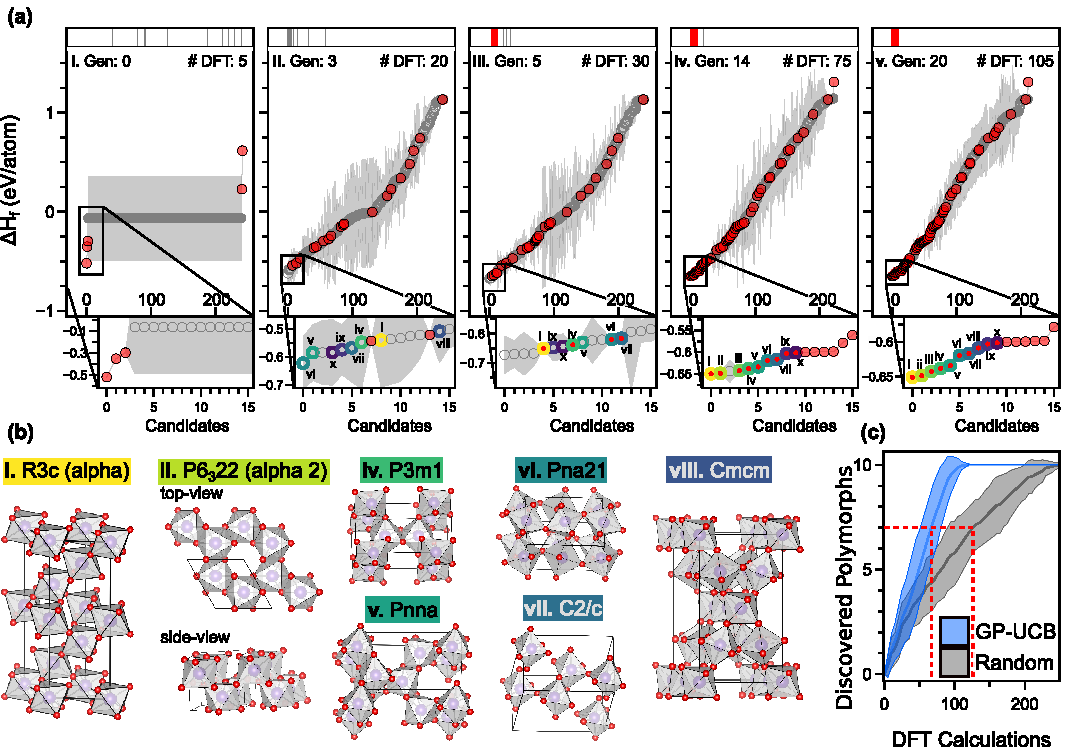
\includegraphics[width=\textwidth,height=\textheight,keepaspectratio]
{02_figures/ml_convergence_plots/test_iro3_al.pdf}
}
\caption{\label{fig:iro2_al}
% (a) %%%%%%%%%%%%%%%%%%%%%%%%%%%%%%%%%%%%%%%%%%%%%%%%%%%%%%%%%%%%%%%%%%%%%%%%%
(a) Progress of the active learning algorithm at five subsequent generations.
%
The AL generation and number of DFT training data at each generation is shown for each subplot.
%
The enthalpy of formation is plotted, ordered from most to least stable, against all \IrOthree candidates.
%
Grey markers indicate predicted formation enthalpies from the ML model while red markers correspond to DFT-computed quantities.
%
Error bars from the GP model corresponding to 1 sigma are shown for all predictions.
%
The vertical lines at the top of each subplot are tracking the positions of the \num{10} most stable polymorphs at each generation and whether they have been acquired (red) or not (grey) by the AL routine.
% (b) %%%%%%%%%%%%%%%%%%%%%%%%%%%%%%%%%%%%%%%%%%%%%%%%%%%%%%%%%%%%%%%%%%%%%%%%%
% (b) Parity plot of the final ML models for \IrOtwo and \IrOthree predicting on either the pre-optimized (grey) or the post-optimized structures of \IrOtwo and \IrOthree.
% (c) %%%%%%%%%%%%%%%%%%%%%%%%%%%%%%%%%%%%%%%%%%%%%%%%%%%%%%%%%%%%%%%%%%%%%%%%%
% (c) Zoomed inset of the 6th generation of the AL loop.
% (d) %%%%%%%%%%%%%%%%%%%%%%%%%%%%%%%%%%%%%%%%%%%%%%%%%%%%%%%%%%%%%%%%%%%%%%%%%
(b) Crystal structures of \num{6} most stable \IrOthree polymorphs.
% (e) %%%%%%%%%%%%%%%%%%%%%%%%%%%%%%%%%%%%%%%%%%%%%%%%%%%%%%%%%%%%%%%%%%%%%%%%%
(c) The number of most stable \num{10} polymorphs of \IrOthree that are discovered as a function of the number of DFT bulk relaxations, averaged over \num{5} independent runs of the AL algorithm using the GP-UCB acquisition criteria (red) and a random acquisition method (grey).
%
Error bars indicate the standard deviation over \num{5} runs.
%
Red guide lines are displayed to show how many DFT calculations are needed to discover \num{7/10} of most stable polymorphs for the GP-UCB and random acquisition.
}
\end{figure*}
% __|
% =========================================================


% =========================================================
% FIGURE ==================================================
% | - Figure | IrO2/3 Parity Plot
\begin{figure*}[!htb]
\centering
\makebox[\textwidth][c]{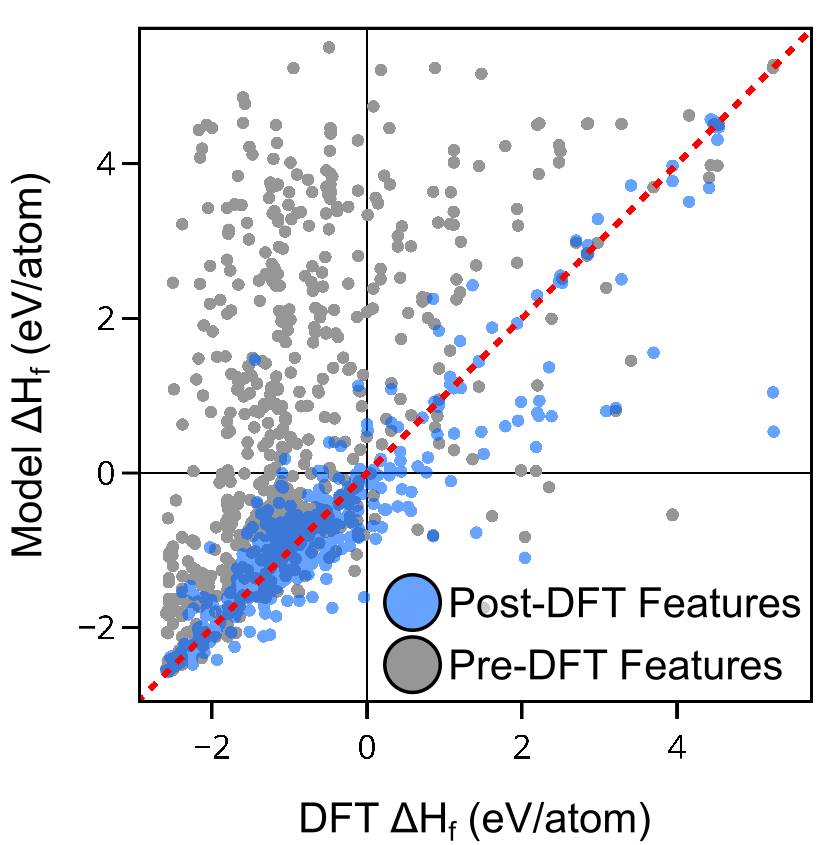
\includegraphics[]
{02_figures/parity_plot.png}
}
\caption{\label{fig:parity}
%
Parity plot of the final ML models for \IrOtwo and \IrOthree predicting on either the pre-optimized (grey) or the post-optimized structures of \IrOtwo and \IrOthree.
}
\end{figure*}
% __|
% =========================================================


% TEMP | Find a place for these sentences where they flow
% The low energy region of Figure~\ref{fig:iro2_al}a.iii is shown in Figure~\ref{fig:iro2_al}c.
%
% And the \num{6} most stable structural polymorphs are shown in Figure~\ref{fig:iro2_al}d. \tetbf{misplaced text}



% | - __old__
% This is clearly seen in the parity plot (Fig TEMP), which shows that the predicted DFT energies become increasingly less accurate as stability of the polymorph decreases, with low stability structures tending to reconfigure into lower energy states.
% %
% This is significantly lower than the leave-one out cross validation error of ~0.15 eV/atom, which is performed by predicting only on optimized structures, indicating that the issue does not lie with a poor predictive model, but instead with the large degree of structural reorganization that occurs over the course of a typical DFT ionic optimization.
% %
% % This is because the candidate space structures are generated
% % To compare the performance of the AL routine we compare against a
% %
% Figure subplot TEMP shows the parity plot of the predicted DFT energies using the fingerprints corresponding to the unoptimized structures (COLOR1) and post-DFT relaxed structures (COLOR2),
% plotted against the final post-optimization DFT formation energy.
% % Sentence that explains the parity plot
% It is clear that the GP model severely underpredicts the energy of the candidate space, especially for systems with less stable predicted formation energies, when predicting onto the candidate space of unoptimized structures (MAE of ~0.5 eV/atom).
% %
% This is due to the fact that the structures undergo through a large degree of structural rearrangement over the course of the DFT relaxation.
% %
% Alternatively, the MAE is much lower when the model predicts onto the post-optimized structures (MAE ~0.15 eV/atom),
% demonstrating that the poor predictive capabilities is due primarily to structural drift and not to the poor predictive capabilities of the GP model.
%
% Despite these shortcomings, Figure TEMP (TEMP performance plot) tracks the number of high stability materials (lowest N structures) discovered as a function of the number of DFT calculations for the case of 1.) AL with UCB acquisition function and 2.) AL with a random acquisition function.
% %
% The random acquisition function emulates the behavior of regression model which exhibits no correlation between the input and output space.
% %
% Clearly, the rate of discovery for case 1.) is superior to that of case 2.), with our methodology discovering half of the lowest N structures after only TEMP DFT calculations compared to TEMP when acquiring randomly within the candidate space.
%
% The middle panel is reproduced in Figure~\ref{fig:iro2_al}, which also shows the real DFT energies accompanying each predicted formation energy (hollow diamonds).
% Probably remove the diamonds and add the parity subplot?
% Figure~\ref{fig:iro2_al} b. shows the formation energy, either predicted (small colored circles) or computed (large red-bordered circles), is plotted on the y-axis against all structures in the candidate space of \IrOthree polymorphs.
%
% As seen from Figure\ref{fig:iro2_al} a) the early iterations, where the training data is sparse
%
% Figure~\ref{fig:iro2_al} a. shows the progression of the model at selected generations of the active learning loop, starting and ending with the initially seeded generation and final generation, respectively.
%
% An acquisition bin size of 10 DFT calculations per iteration and an initial seed of 11 calculations were used.
% plots of the AL predictions on the candidate space at particular generations of the AL algorithm for the \IrOthree candidate space with an acquisition bin size of 10 DFT calculations per iteration and an initial 11 calculations used for seeding.
% The AL algorithm is applied separately to \IrOtwo and \IrOthree because we are specifically interested in the most stable polymorphs at each stoichiometry.
% TODO How many features drop out when you constrain the stoich.?
% This has an the added benefit of reducing the number of fingerprint vectors from the Voronoi tesselation dramatically (from TEMP to TEMP) because many features are senstive to changes in stoichiometry.
% __|
